\section{Supplementary material}\label{sec:app}

\begin{figure}[h]
	\centering
	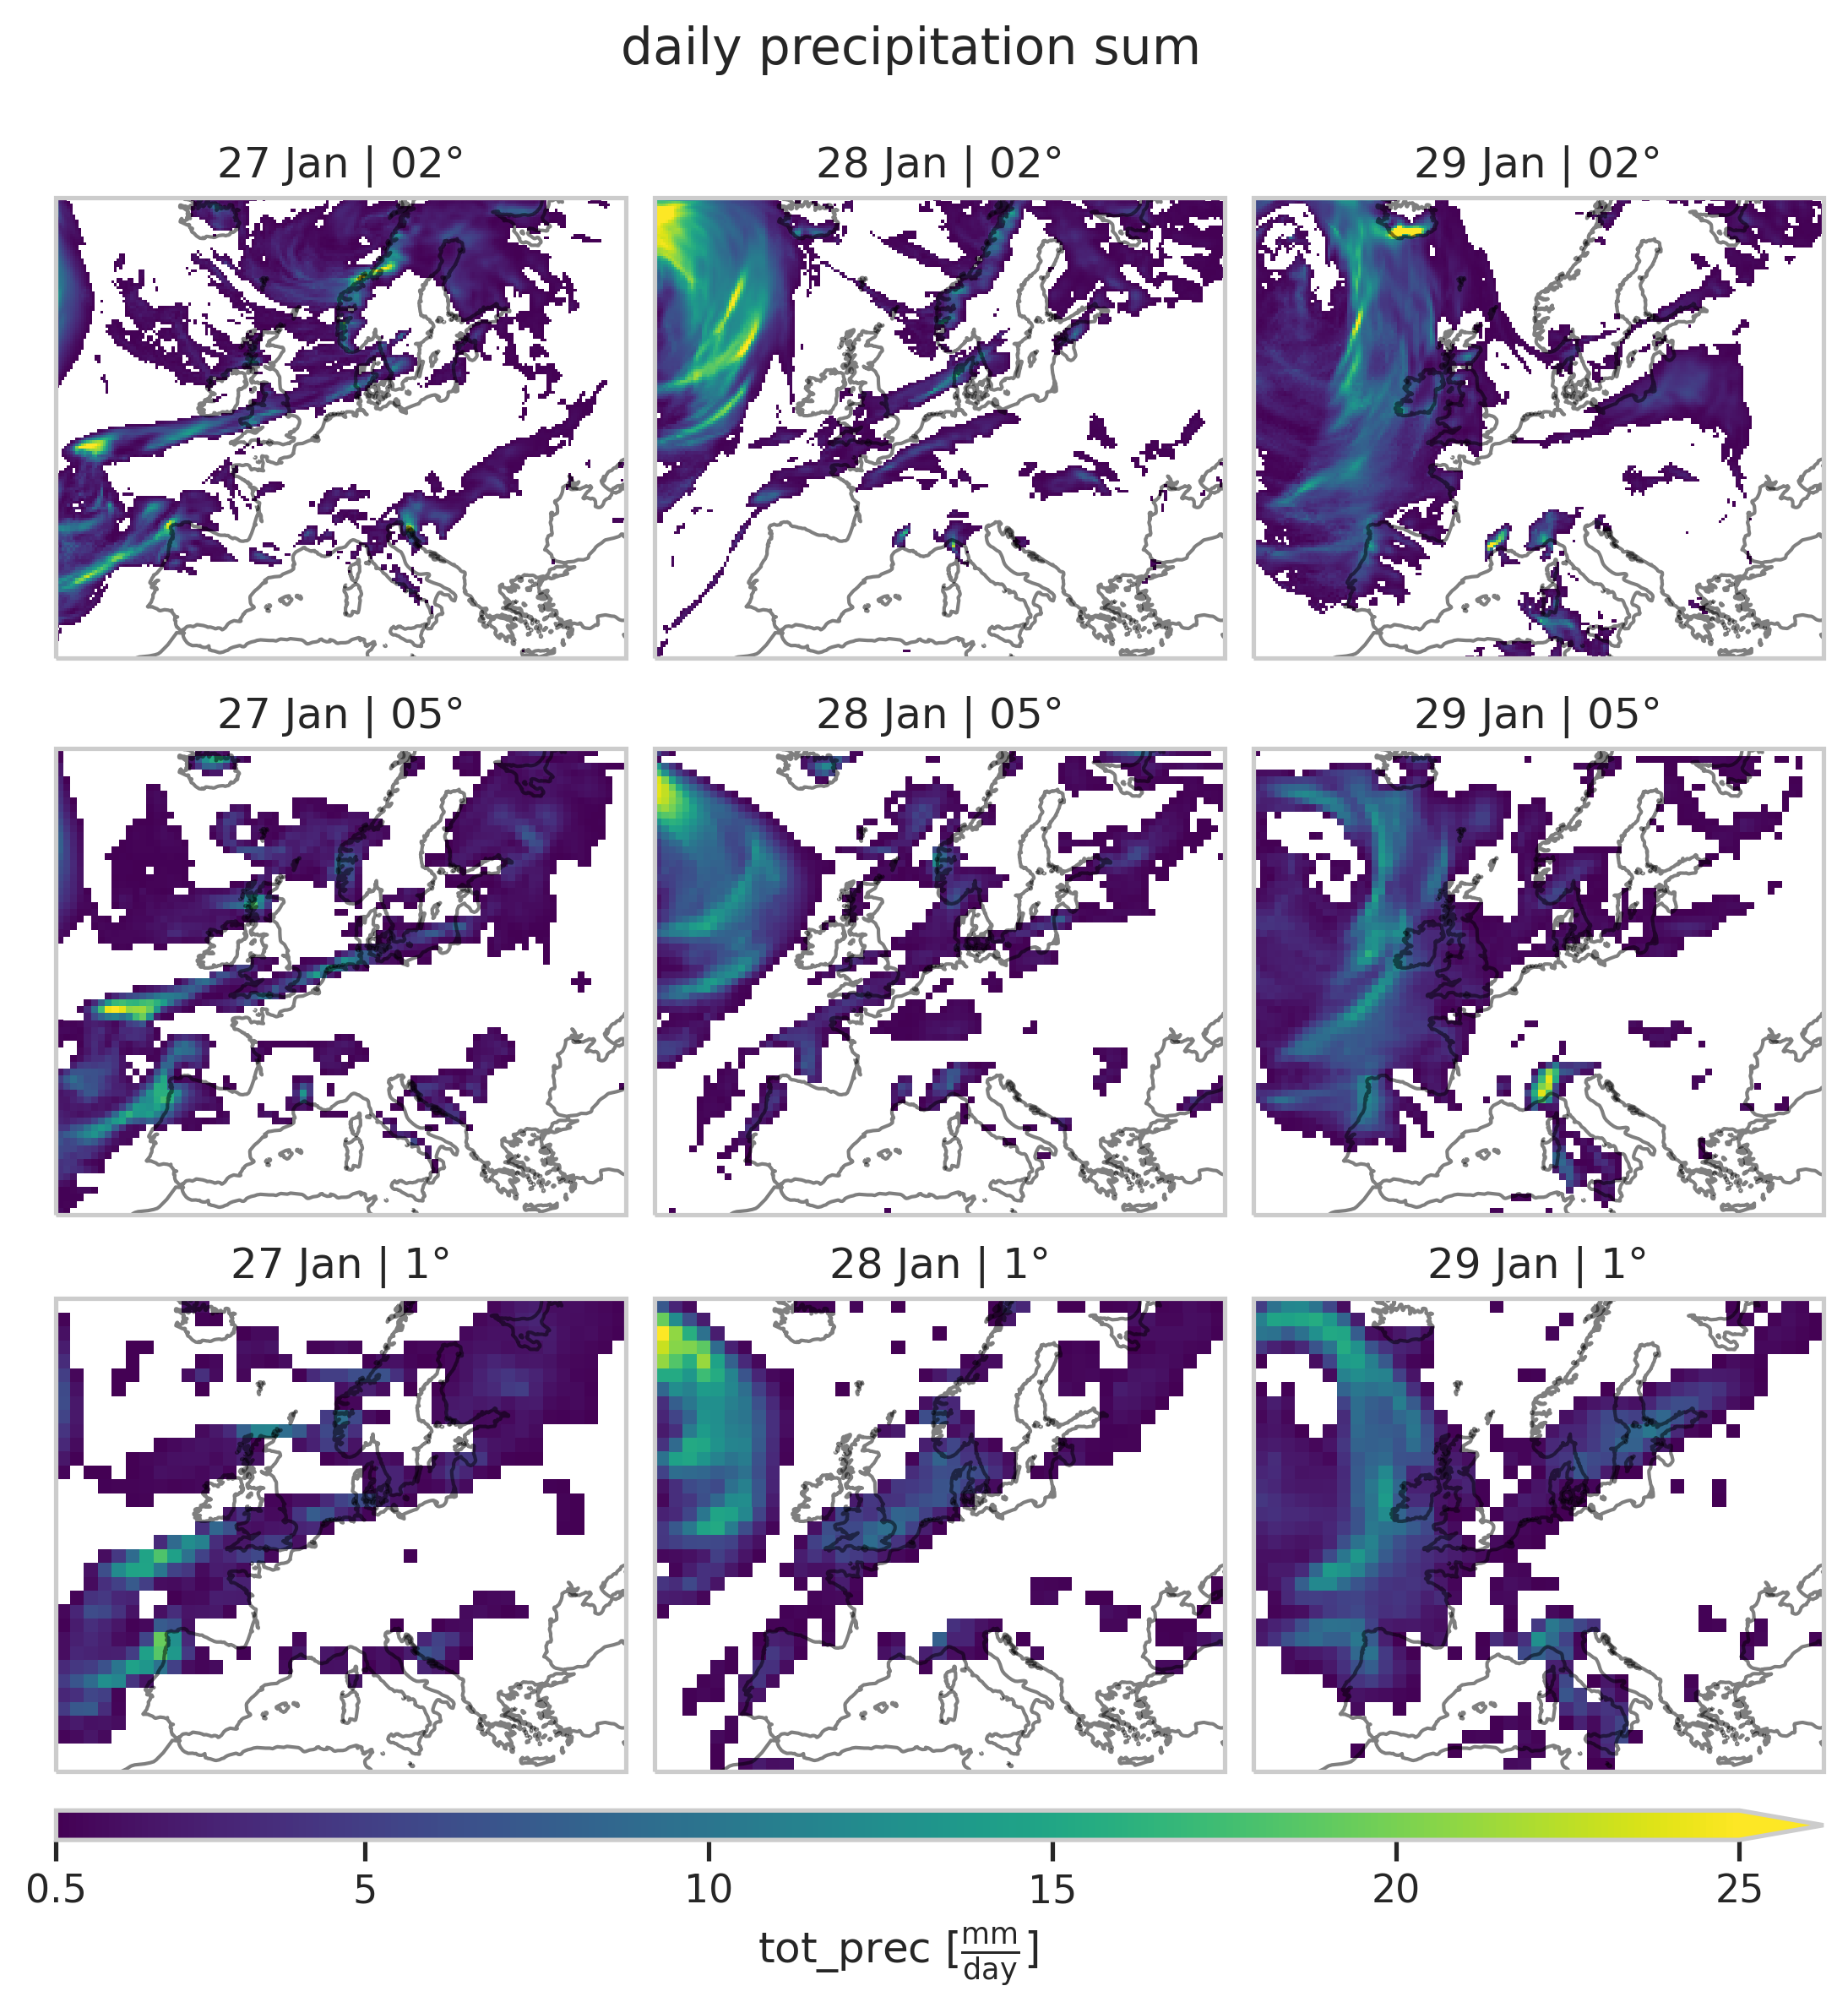
\includegraphics[width=0.7\figwidth]{../figs/6-event.png}
	\caption{Maps of daily precipitation sum during event from 27 to 29 Jan (shortly after \href{https://en.wikipedia.org/wiki/Burns\%27_Day_Storm}{Cyclone \textit{Daria}}). Identical grid resolutions are displayed row-wise, while columns represent single days. Precipitation below \SI{0.5}{\mm\per\day} is excluded. When focussing on the differences among grid resolutions, it is notable that (a) 1°-resolution displays large areas of precipitation in Northeastern Europe, while (b) 0.2°-resolution rather shows high intensities over the Atlantic Ocean and Iceland. Interestingly, solely 0.5°-resolution captures \textit{strong} precipitation event over south-western Alps on 29 Jan, which indicates the complexity of assessing effects of changing grid resolution.}
	\label{fig:app-event}
\end{figure}